\documentclass{./../../Latex/teaching_slides}
\usepackage{venndiagram}
\usepackage{tikz}
\usepackage{pgfplots}
\usetikzlibrary{arrows.meta}

\begin{document}

\title{ECON 441 \\ \vspace{0.4em} \normalsize Introduction to Mathematical Economics}
\author{Div Bhagia}
\date{Lecture 3: Linear Algebra}

%%%%%%%%%%%%%%% 
\begin{frame}[noframenumbering, plain]
\maketitle
\end{frame}


%%%%%%%%%%%%%%% 
\begin{frame}{Inverse of a Matrix}
For a \textbf{square} matrix $A$, it's inverse $A^{-1}$ is defined as:
$$
A A^{-1}=A^{-1} A=I
$$

\vspace{2em}
 Squareness is a \textit{necessary} condition not a \textit{sufficient} condition \\~\\
 If a matrix's inverse exists, it's called a \textbf{nonsingular} matrix
\end{frame}

%%%%%%%%%%%%%%% 
\begin{frame}{Inverse of a Matrix}
If an inverse exists, it is unique. \\~\\
Proof by contradiction. Let's say $B = A^{-1}$ and $C=A^{-1}$.
Then, $$ AB=BA=I $$
 $$ AC=CA=I $$
Pre-multiply both sides by $B$,
$$ BAC=BCA=BI  \implies C=B $$
\end{frame}

%%%%%%%%%%%%%%% 
\begin{frame}{Solution of Linear-Equation System}
$$ Ax = b $$

\vspace{1em}
Pre-multiply both sides by $A^{-1}$, 
$$ A^{-1} Ax = A^{-1} b \quad \implies x = A^{-1} b $$

If $A$ is singular, a unique solution does not exist. 
\end{frame}

%%%%%%%%%%%%%%% 
\begin{frame}{Conditions for Nonsingularity}
Squareness is \textit{necessary} but not  \textit{sufficient} \\~\\
Sufficient condition for nonsingularity: \\~\\
\hspace{1em} \textit{Rows (or equivalently) columns are linearly independent} \\~\\
Example. $$
A=\left[\begin{array}{ll}
1 & 2 \\
2 & 4
\end{array}\right]
\quad
B=\left[\begin{array}{ll}
1 & 2 \\
3 & 4
\end{array}\right]
$$
\pause $A$ is singular, $B$ is nonsingular.
\end{frame}

%%%%%%%%%%%%%%% 
\begin{frame}{Linear Independence}
\begin{columns}[T]
\begin{column}{0.5\textwidth}
\centering
Linearly Dependent \\ \vspace{0.5em}
	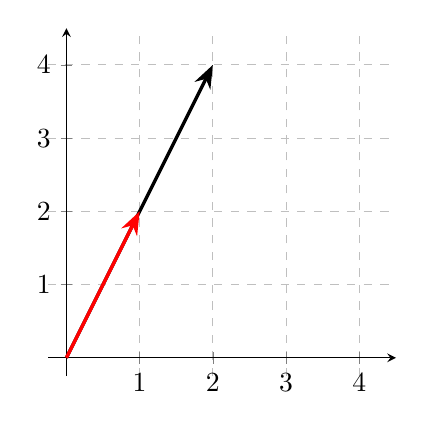
\begin{tikzpicture}
\begin{axis}[
    axis lines=middle, % Places the axis in the middle
    xlabel={},
    ylabel={},
	xtick = {1, 2, 3, 4}, 
	ytick = {1, 2, 3, 4}, 
    xmin=-0.25, xmax=4.5, 
    ymin=-0.25, ymax=4.5, 
    grid style=dashed,
    grid=both, 
    width=6cm, height=6cm, 
    vector/.style={-Stealth, red, very thick} 
]
\addplot[vector, black] coordinates {(0,0) (2,4)};
\addplot[vector] coordinates {(0,0) (1,2)};
\end{axis}
\end{tikzpicture}
\end{column}	
\begin{column}{0.5\textwidth}
\centering
Linearly Independent \\ \vspace{0.5em}
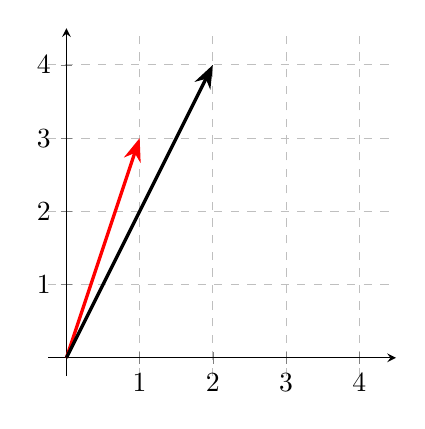
\begin{tikzpicture}
\begin{axis}[
    axis lines=middle, % Places the axis in the middle
    xlabel={},
    ylabel={},
	xtick = {1, 2, 3, 4}, 
	ytick = {1, 2, 3, 4}, 
    xmin=-0.25, xmax=4.5, 
    ymin=-0.25, ymax=4.5, 
    grid style=dashed,
    grid=both, 
    width=6cm, height=6cm, 
    vector/.style={-Stealth, red, very thick} 
]
\addplot[vector] coordinates {(0,0) (1,3)};
\addplot[vector, black] coordinates {(0,0) (2,4)};
\end{axis}
\end{tikzpicture} 
\end{column}	
\end{columns}
\end{frame}

%%%%%%%%%%%%%%% 
\begin{frame}{Conditions for Nonsingularity}
$$
A=\left[\begin{array}{ll}
1 & 2 \\
2 & 4
\end{array}\right]
\quad  x=\left[\begin{array}{ll}
x_1 \\
x_2
\end{array}\right]
\quad d=\left[\begin{array}{ll}
a \\
b
\end{array}\right]
$$
\vspace{1em}

We have a system of linear equations:
$$ Ax = d $$
Then, 
$$ x_1+2x_2 = a $$
$$ 2x_1+4x_2 = b $$
\end{frame}

%%%%%%%%%%%%%%% 
\begin{frame}{Conditions for Nonsingularity}
$$ x_1+2x_2 = a $$
$$ 2x_1+4x_2 = b $$
For these equations to be consistent, we need $b=2a$:
$$ x_1+2x_2 = a $$
$$ 2x_1+4x_2 = 2a $$
Both are the same equation, infinite number of solutions.
\end{frame}

%%%%%%%%%%%%%%% 
\begin{frame}{Conditions for Nonsingularity}
\vspace{1em}

To summarize, for a matrix to be nonsingular (i.e. its inverse exists): \\~\\

Necessary condition: \textbf{Squareness} \\~\\

Sufficient condition: \textbf{Rows or (equivalently) columns are linearly independent} 

\end{frame}


%%%%%%%%%%%%%%% 
\begin{frame}{Rank of a Matrix}
Rank of a matrix $=$ maximum number of linearly independent rows \\~\\
$$A=\left[\begin{array}{ll}
1 & 2 \\
3 & 4
\end{array}\right]
\quad
B=\left[\begin{array}{ll}
1 & 2 \\
2 & 4
\end{array}\right]
$$
\vspace{1em}

Rank of $A$? Rank of $B$? \\~\\
\pause
Full rank $ \iff $ Nonsingularity
\end{frame}

%%%%%%%%%%%%%%% 
\begin{frame}{Checking for Linear Independence}
\textit{Echelon} form of a matrix. \\~\\
\begin{witemize}
\item First row: all elements \textit{can be} non-zero
\item Second row: first element $0$
\item Third row: first two elements $0$
$$\vdots$$
\item Last row: first $m-1$ elements zero
\end{witemize}
\end{frame}

%%%%%%%%%%%%%%% 
\begin{frame}{Checking for Linear Independence}
\textit{Echelon} form of a $2 \times 2$ matrix. \\~\\
$$
A=\left[\begin{array}{ll}
a_{11} & a_{12} \\
\red{0} & a_{22}
\end{array}\right]
$$
\end{frame}

%%%%%%%%%%%%%%% 
\begin{frame}{Checking for Linear Independence}
\textit{Echelon} form of a $3 \times 3$ matrix. \\~\\
$$
A=\left[\begin{array}{ccc}
a_{11} & a_{12} & a_{13} \\
\red{0} & a_{22} & a_{23}  \\
\red{0} & \red{0} & a_{33}
\end{array}\right]
$$
\end{frame}

%%%%%%%%%%%%%%% 
\begin{frame}{Checking for Linear Independence}
Valid operations to convert to echelon form:\\~\\
\begin{witemize}
\item Interchange any two rows
\item Multiplication (or division) of a row by a scalar $k \neq 0$
\item Addition of a (or $k$ times of a) row to another \\~\\
\end{witemize}
\end{frame}

%%%%%%%%%%%%%%% 
\begin{frame}{Converting to Echelon Form}
Given matrix:
$$ A= \left[\begin{array}{ccc}
a_{11} & a_{12} & a_{13} \\
a_{21} & a_{22} & a_{23}  \\
a_{31} & a_{32} & a_{33}
\end{array}\right] $$
\vspace{1em}

Target elements in order:
$$
\left[\begin{array}{ccc}
b_{11} & b_{12} & b_{13} \\
b_{21} & b_{22} & b_{23}  \\
\red{0} & b_{32} & b_{33}
\end{array}\right] \rightarrow
\left[\begin{array}{ccc}
c_{11} & c_{12} & c_{13} \\
\red{0} & c_{22} & c_{23}  \\
\red{0} & c_{32} & c_{33}
\end{array}\right] \rightarrow
\left[\begin{array}{ccc}
d_{11} & d_{12} & d_{13} \\
\red{0} & d_{22} & d_{23}  \\
\red{0} & \red{0} & d_{33}
\end{array}\right]
$$
\end{frame}


%%%%%%%%%%%%%%% 
\begin{frame}{Checking for Linear Independence}
Convert to \textit{echelon} form to check for linear independence. \\~\\
Example. $$
A=\left[\begin{array}{ccc}
0 & -1 & -4 \\
3 & 1 & 2 \\
6 & 1 & 0
\end{array}\right]
$$
\end{frame}

%%%%%%%%%%%%%%% 
\begin{frame}{Checking for Linear Independence}
\textit{Echelon} form, similar to solving by substitution. \\~\\
In our original example, 
$$A = \begin{bmatrix}
1 & 2 \\
1 & -3 
\end{bmatrix} \quad 
x = \begin{bmatrix}
q \\
p 
\end{bmatrix} \quad 
b = \begin{bmatrix}
100 \\
20 
\end{bmatrix}$$
\end{frame}

%%%%%%%%%%%%%%% 
\begin{frame}{Checking for Linear Independence}
Consider augmented matrix:
$$ A=\left[\begin{array}{cc|c}1 & 2 & 100 \\ 1 & -3 & 20\end{array}\right] $$
Reduce to echelon form:
$$ A=\left[\begin{array}{cc|c}1 & 2 & 100 \\ 0 & -5 & -80\end{array}\right] $$

$$ q+2p = 100 \quad \quad -5p = -80   $$
\end{frame}

%%%%%%%%%%%%%%%% 
\begin{frame}{Checking for Nonsingularity}
Rank of a matrix $=$ maximum number of linearly independent rows or (equivalently) columns \\~\\

If a square matrix has full rank, it is nonsingular. \\~\\

To check for nonsingularity or finding rank: echelon form. \\~\\

Alternatively, calculate the \textbf{determinant} to check for nonsingularity. For singular matrices, the determinant is zero. 
\end{frame}

%%%%%%%%%%%%%%%% 
 \begin{frame}{Determinant}
 Determinant $|A|$ is a unique scalar associated with a \textit{square} matrix $A$. \\~\\
 Determinant of a $2 \times 2$ Matrix:
 $$ A=\left[\begin{array}{ll}a_{11} & a_{12} \\ a_{21} & a_{22}\end{array}\right] $$
 Can be calculated as:
 $$ |A|=a_{11} a_{22}-a_{12} a_{21} $$  
 \end{frame}

%%%%%%%%%%%%%%%% 
 \begin{frame}{Determinant: Geometric Interpretation}
 
\begin{columns}[T]
\begin{column}{0.25\textwidth}
  	 $$ A=\left[\begin{array}{ll}1 & 2 \\ 3 & 4\end{array}\right] $$ 
\end{column}	
\begin{column}{0.75\textwidth}
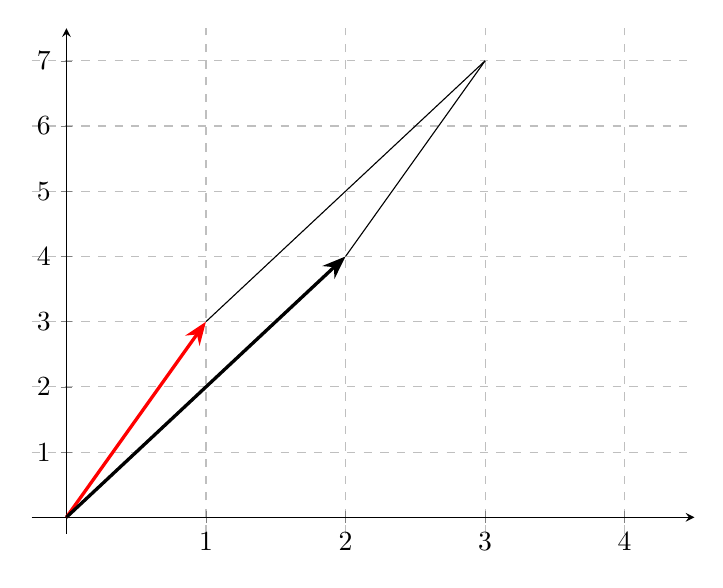
\begin{tikzpicture}
\begin{axis}[
    axis lines=middle, % Places the axis in the middle
    xlabel={},
    ylabel={},
	xtick = {1, 2, 3, 4}, 
	ytick = {1, 2, 3, 4, 5, 6, 7}, 
    xmin=-0.25, xmax=4.5, 
    ymin=-0.25, ymax=7.5, 
    grid style=dashed,
    grid=both, 
    width=10cm, height=8cm, 
    vector/.style={-Stealth, red, very thick} 
]
\addplot[vector] coordinates {(0,0) (1,3)};
\addplot[vector, black] coordinates {(0,0) (2,4)};
\addplot[solid, black] coordinates {(1,3) (3,7)};
\addplot[solid, black] coordinates {(2,4) (3,7)};
\end{axis}
\end{tikzpicture}
\end{column}	
\end{columns}

 \end{frame}

%%%%%%%%%%%%%%%% 
 \begin{frame}{Determinant of a $3 \times 3$ Matrix}
$$
\begin{aligned}
|A| &=\left|\begin{array}{lll}
a_{11} & a_{12} & a_{13} \\
a_{21} & a_{22} & a_{23} \\
a_{31} & a_{32} & a_{33}
\end{array}\right| \\~\\
&=a_{11}\left|\begin{array}{ll}
a_{22} & a_{23} \\
a_{32} & a_{33}
\end{array}\right|-a_{12}\left|\begin{array}{ll}
a_{21} & a_{23} \\
a_{31} & a_{33}
\end{array}\right| 
+a_{13}\left|\begin{array}{ll}
a_{21} & a_{22} \\
a_{31} & a_{32}
\end{array}\right|
\end{aligned}
$$
 \end{frame}
 
%%%%%%%%%%%%%%%% 
 \begin{frame}{Determinant of a $n \times n$ Matrix}
A \textit{minor} of the element $a_{ij}$, denoted by $|M_{ij}|$ is obtained by deleting the $i$th row and $j$th column. \\~\\
Cofactor $C_{ij}$ is defined as:
$$ |C_{ij}| = (-1)^{i+j} |M_{ij}| $$
 Then, 
 $$|A| = \sum_{i=1}^n a_{ij} |C_{ij}| = \sum_{j=1}^n a_{ij} |C_{ij}| $$
 \end{frame}

 
%%%%%%%%%%%%%%% 
\begin{frame}{References and Homework Problems}
\begin{witemize}
\item New references for today: 5.1, 5.2
\item Homework problems: \\
\begin{witemize}
\normalsize
\item Exercise 5.1: 3, 4, 5, 6
\item Exercise 5.2: 1 (c) (e) (f), 2, 3, 6
\end{witemize}

\end{witemize}
\end{frame}






\end{document}